\documentclass[12pt,a4paper,oneside]{article}
\usepackage[a4paper,total={160mm,250mm}]{geometry}
\usepackage[utf8]{inputenc}
\usepackage[T1]{fontenc}
\usepackage{amsmath}
\usepackage{amsfonts}
\usepackage{amssymb}
\usepackage{amsthm}
\usepackage{comment}
\usepackage{graphicx}
\usepackage{enumerate}
%\usepackage[printsolution=true]{exercises}
\usepackage{tasks}
\usepackage{tcolorbox}
\usepackage{marginnote}
\usepackage{mdframed}
\usepackage{multicol}
\usepackage{mhchem}

\usepackage{tikz}
\usetikzlibrary{matrix}

\newcommand{\annotation}[1]{\reversemarginpar\marginpar{\small\itshape\color{blue}{#1}}}

\setlength{\columnseprule}{1pt}

\newcommand{\hide}{0}
\newcommand{\hideif}[1]{\if\hide1\phantom{#1}\else {#1}\fi}

\includecomment{solutions}
%\excludecomment{solutions}

%\pagenumbering{gobble}
\setlength{\parindent}{0pt}

%\theoremstyle{definition}
%\newtheorem*{example*}{Example}
%
%\theoremstyle{definition}
%\newtheorem{example}{Example}
%
%\theoremstyle{definition}
%\newtheorem{exercise}{Exercise}
%
%\theoremstyle{definition}
%\newtheorem*{solution*}{Solution}

\newcounter{taskcounter}
\numberwithin{taskcounter}{section}

\newenvironment{exercise}{%
	\refstepcounter{taskcounter}
	\mdfsetup{%
		frametitle={%
			\tikz[baseline=(current bounding box.east),outer sep=0pt]
			\node[anchor=east,rectangle,fill=blue!20]
			{\strut Exercise~\thetaskcounter};
		}
	}
	\mdfsetup{%
		innertopmargin=5pt,linecolor=blue!20,%
		linewidth=2pt,topline=true,roundcorner=5pt,%
		frametitleaboveskip=\dimexpr-\ht\strutbox\relax%
	}
	\begin{mdframed}[nobreak=false]\relax
	}{%
	\end{mdframed}
}

\newenvironment{example}{%
	\refstepcounter{taskcounter}
	\mdfsetup{%
		frametitle={%
			\tikz[baseline=(current bounding box.east),outer sep=0pt]
			\node[anchor=east,rectangle,fill=green!20]
			{\strut Example~\thetaskcounter};
		}
	}
	\mdfsetup{%
		innertopmargin=5pt,linecolor=green!20,%
		linewidth=2pt,topline=true,roundcorner=5pt,%
		frametitleaboveskip=\dimexpr-\ht\strutbox\relax%
	}
	\begin{mdframed}[nobreak=false]\relax
	}{%
	\end{mdframed}
}

\newenvironment*{solution*}{%
	\mdfsetup{%
		frametitle={%
			\tikz[baseline=(current bounding box.east),outer sep=0pt]
			\node[anchor=east,rectangle,fill=cyan!20]
			{\strut Solution};
		}
	}
	\mdfsetup{%
		innertopmargin=5pt,linecolor=cyan!20,%
		linewidth=2pt,topline=true,roundcorner=5pt,%
		frametitleaboveskip=\dimexpr-\ht\strutbox\relax%
	}
	\begin{mdframed}[nobreak=false]\relax
	}{%
	\end{mdframed}
}

\begin{document}
	\section*{Introduction: Exponential Growth}
%Before we look at exponential growth, let us recall the familiar concept of \textit{linear growth}.
\begin{example}[linear growth] \label{ex:linear_growth}
	Suppose we have a bank account with 50 CHF at the beginning of year zero.
	At the end of every year, we deposit 20 CHF.
	How much money are we going to have at the beginning of year $x$?
	The answer clearly is $20x+50$ CHF.
	This is visulaized in Figure~\ref{ex:linear_growth} (left).
	Also, we can fill the amount of money at the beginning of each year into a table.
%	\begin{table}[ht]
%		\centering
%		\begin{tabular}{|l|c|c|c|c|c|c|c|c|c|} \hline
%			year & 0 & 1 & 2 & 3 & 4 & 5 & 6 & 7 & 8 \\ \hline
%			CHF & 50 & 70 & 90 & 110 & 130 & 150 & 170 & 190 & 210 \\ \hline
%		\end{tabular}
%		\label{tab:linear_growth}
%	\end{table}
	\begin{figure}[ht]
	\centering
	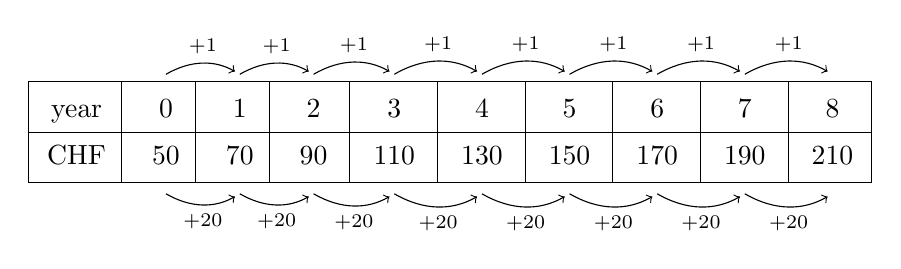
\begin{tikzpicture}
		\matrix[matrix of math nodes,draw, column sep=1em,row sep=.5mm] (mx) {
			\textrm{year} & 0 & 1 & 2 & 3 & 4 & 5 & 6 & 7 & 8 \\
			\textrm{CHF} & 50 & 70 & 90 & 110 & 130 & 150 & 170 & 190 & 210 \\
		};
		\path[->,shorten >=2pt]
		\foreach \from/\to in {2/3,3/4,4/5,5/6,6/7,7/8,8/9,9/10} {
			([yshift=2mm]mx-1-\from.north) edge[bend left]
			node[above] {$\scriptstyle+1$} ([yshift=2mm]mx-1-\to.north)
			([yshift=-2.5mm]mx-2-\from.south) edge[bend right]
			node[below] {$\scriptstyle+20$} ([yshift=-2.5mm]mx-2-\to.south)
		};
		\foreach \x in {2,...,10}{
			\draw ([xshift=-1em]mx.north west -| mx-1-\x.west) -- ([xshift=-1em]mx.south west -| mx-1-\x.west);
		};
		\draw (mx.west) -- (mx.east);
	\end{tikzpicture}
	\end{figure}
\end{example}
\annotation{5}
\begin{exercise} \label{ex:exponential_growth}
	Suppose we have again a bank account with 50 CHF at the beginning of year zero.
	But now, we will not deposit any additional money.
	Instead, the bank pays us an intrest of 20\% at the end of each year.
	So if we have 100 CHF on our bank account during a certain year, then the bank will pay us 20 CHF (i.e. 20\%) at the end of that year.
	\begin{tasks}
		\task How much money are we going to have at the beginning of year $x$? Create and fill a table analogusly to the one in Example~\ref{ex:linear_growth}.
		\task Find a function $f\left(x\right)$ that returns the amount of money at the end of year $x$.
		\task Draw the graph of the function $f\left(x\right)$ and compare it to the one in Example~\ref{ex:linear_growth}.
	\end{tasks}
\end{exercise}
\begin{solution*}
	At the end of year zero, we have 50 CHF on our bank account.
	Consequently, at the beginning of year one, we will have $60=50\cdot 1.2$ CHF.
	At the end of year two, we have $72=60\cdot 1.2$ CHF.
	This can also bewritten as $72=50\cdot 1.2^2$ CHF.
	Following this scheme, we arrive at the solution given below.
	\begin{enumerate}[a)]
		\item The table is given by
%		\begin{tabular}{|l|c|c|c|c|c|c|c|c|c|} \hline
%			year & 0 & 1 & 2 & 3 & 4 & 5 & 6 & 7 & 8 \\ \hline
%			CHF & 50 & 60 & 72 & 86.4 & 103.68 & 124.416 & 149.2992 & 179.15904 & 214.990848 \\ \hline
%		\end{tabular}\\
		\begin{figure}[ht]
			\centering
			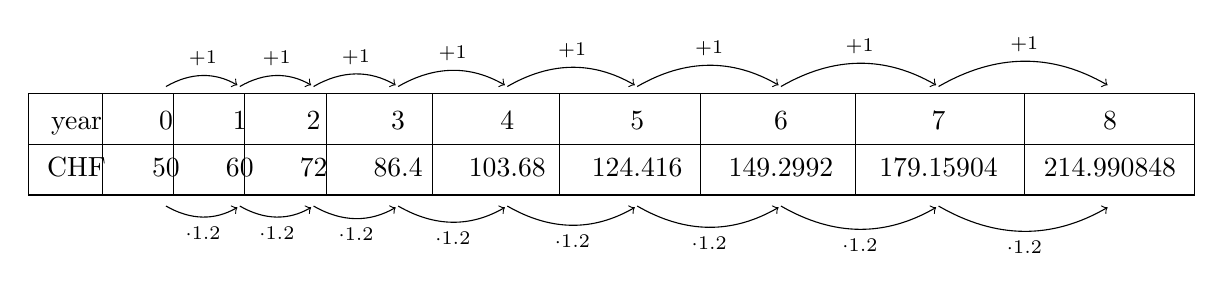
\begin{tikzpicture}
				\matrix[matrix of math nodes,draw, column sep=1em,row sep=.5mm] (mx) {
					\textrm{year} & 0 & 1 & 2 & 3 & 4 & 5 & 6 & 7 & 8 \\
					\textrm{CHF} & 50 & 60 & 72 & 86.4 & 103.68 & 124.416 & 149.2992 & 179.15904 & 214.990848 \\
				};
				\path[->,shorten >=1pt]
				\foreach \from/\to in {2/3,3/4,4/5,5/6,6/7,7/8,8/9,9/10} {
					([yshift=2mm]mx-1-\from.north) edge[bend left]
					node[above] {$\scriptstyle+1$} ([yshift=2mm]mx-1-\to.north)
					([yshift=-2.5mm]mx-2-\from.south) edge[bend right]
					node[below] {$\scriptstyle\cdot 1.2$} ([yshift=-2.5mm]mx-2-\to.south)
				};
				\foreach \x in {2,...,10}{
					\draw ([xshift=-\x-15]mx.north west -| mx-1-\x.west) -- ([xshift=-\x-15]mx.south west -| mx-1-\x.west);
				};
				\draw (mx.west) -- (mx.east);
			\end{tikzpicture}
		\end{figure}
		\item The function is given by $f\left(x\right)=50\cdot 1.2^x$ CHF.
		\item The graph of $f\left(x\right)$ is given in Figure~\ref{fig:linear_exponential_growth} (right).
	\end{enumerate}
\end{solution*}
\begin{figure}[ht]
	\centering
	\includegraphics[width=0.45\textwidth]{images/linear_growth}\hfill
	\includegraphics[width=0.45\textwidth]{images/quadratic_growth}
	\caption{An example of linear growth (left) and exponential growth (right).}
	\label{fig:linear_exponential_growth}
\end{figure}
\annotation{20}
\begin{tcolorbox}
	We say that a function $f\left(x\right)$ grows \ldots
	\begin{itemize}
		\item[] \ldots\ \textbf{linearly}, if $f\left(x\right)=ax+b$ for some $a>0$, and \ldots
		\item[] \ldots\ \textbf{exponentially}, if $f\left(x\right)=a\cdot b^x$ for some $a>0$ and $b>1$.
	\end{itemize}
\end{tcolorbox}
\begin{example}
	The function in Exercise~\ref{ex:exponential_growth} grows \textit{exponentially} with $a=50$ CHF and $b=1.2$.
\end{example}
\begin{exercise} \label{ex:first_exponential_equation}
	This time, we have only 20 CHF on our bank account at year zero.
	The bank still pays in intrest of 20\% at the end of each year.
	How many years will it take until we have more than 500 CHF on our bank account?
\end{exercise}
\begin{solution*}
	At the beginning of year $x$, we have $f\left(x\right)=80\cdot 1.2^x$ CHF on our bank account.
	We have $f\left(10\right)=495.34$ CHF and $f\left(11\right)=594.41$ CHF (both rounded to two digits).
	Hence it takes 11 years.
\end{solution*}
\annotation{30}
In Exercise~\ref{ex:first_exponential_equation}, we have solved our first \textit{exponential equation}, i.e. an equation where the unknown $x$ occurs in the exponent.
In the next chapter, we develop a more sytematic approach to solve exponential equations.\newpage
	\section*{Solving Equations}
We recall the basic laws for rational exponents:
\begin{tcolorbox}
	For bases $a,b\in\mathbb R$, exponents $x,y\in\mathbb Q$ and $n\in\mathbb N$, we have the following rules:
	\begin{multicols}{3}
		\centering
		\textbf{same base}\\
		\begin{align*}
			a^x\cdot a^y&=a^{x+y} \\[8pt]
			\frac{a^x}{a^y}&=a^{x-y} \\[8pt]
			\left(a^x\right)^y&=a^{x\cdot y}
		\end{align*}
		\vfill
		\columnbreak
		
		\textbf{same exponent}\\
		\begin{align*}
			\left(a\cdot b\right)^x&=a^x\cdot b^x \\[8pt]
			\left(\frac{a}{b}\right)^x&=\frac{a^x}{b^x}
		\end{align*}
		\vfill
		\columnbreak
		
		\textbf{definitions}\\
		\begin{align*}
			a^0&=1 \\[8pt]
			a^{-x}&=\frac{1}{a^x} \\[8pt]
			a^{\frac{1}{n}}&=\sqrt[n]{a}
		\end{align*}
		\vfill
	\end{multicols}
	Note that $x$ and $y$ can now be fractions of integers, for example $x=\frac{m}{n}$.
\end{tcolorbox}
%\begin{tcolorbox}
%	\begin{align*}
%		a^x\cdot a^y&=a^{x+y}&\text{(same base)}\\
%		a^x\cdot b^x&=\left(a\cdot b\right)^x&\text{(same exponent)}\\
%		\left(a^x\right)^y&=a^{x\cdot y}&\text{(exponent of a power)}\\
%		a^{-x}&=\frac{1}{a^x}&\text{(negative exponent)}\\
%		a^{\frac{1}{n}}&=\sqrt[n]{a}&\text{(root)}
%	\end{align*}
%\end{tcolorbox}
These rules can be used to solve equations involving powers.
\begin{exercise}
	Determine all solutions:
	\begin{tasks}(3)
		\task $x^3=-64$
		\task $x^4=10^{-4}$
		\task $x^6=729$
		\task $x^3=1000$
		\task $x^{-6}=729$
		\task $x^{-\frac{5}{2}}=3^{\frac{5}{2}}$
	\end{tasks}
\end{exercise}
\annotation{6}
\begin{tcolorbox}
	\textbf{Exponential equations:} The unknown $x$ occurs in the exponent.
	\begin{itemize}
		\item exponential equations: $2^x=16$ and $3^{x+2}=\frac{1}{27}$
		\item \textbf{not} exponential equations: $x^2=16$ and $\left(x+2\right)^3=\frac{1}{27}$
	\end{itemize}
	Solving exponential equations:
	\begin{enumerate}[Step 1:]
		\item Express both sides as in terms of the same base.
		\item Compare the exponents.
	\end{enumerate}
\end{tcolorbox}
\begin{exampleenv}
\begin{example}
	\begin{minipage}{0.45\textwidth}
		\begin{align*}
			\textrm{a)}\quad 2^x&=16 \\
			2^x&=2^4 \\
			x&=4 \\
			\phantom{x+2}& \\
			\phantom{x+2}&
		\end{align*}
	\end{minipage}\hfill
	\begin{minipage}{0.45\textwidth}
		\begin{align*}
			\textrm{b)}\quad 3^{x+2}&=\frac{1}{27} \\
			3^{x+2}&=3^{-3} \\
			x+2&=-3 \\
			x&=-5
		\end{align*}
	\end{minipage}
\end{example}
\annotation{10}
\end{exampleenv}
\begin{exercise}
	Solve for $x$.
	\begin{tasks}(4)
		\task $2^x=2$ \task $2^x=4$ \task $3^x=27$ \task $2^x=1$
		\task $2^x=\frac{1}{2}$ \task $3^x=\frac{1}{3}$ \task $2^x=\frac{1}{8}$ \task $2^{x+1}=8$
		\task $2^{x-2}=\frac{1}{4}$ \task $3^{x+1}=\frac{1}{27}$ \task $2^{x+1}=64$
		\task $2^{1-2x}=\frac{1}{2}$
	\end{tasks}
\end{exercise}
\annotation{17}
%\begin{exercise}
%	Solve for $x$.
%	\begin{tasks}(4)
%		\task $2^x=32$
%		\task $5^x=25$
%		\task $3^x=81$
%		\task $7^x=1$
%		\task $3^x=\frac{1}{3}$
%		\task $2^x=\sqrt{2}$
%		\task $5^x=\frac{1}{125}$
%		\task $4^{x+1}=64$
%	\end{tasks}
%\end{exercise}
%\annotation{25}
\begin{exercise}
	Solve for $x$.
	\begin{tasks}(4)
		\task $8^x=32$
		\task $4^x=\frac{1}{8}$
		\task $9^x=27$
		\task $25^x=\frac{1}{5}$
		\task $27^x=\frac{1}{9}$
		\task $16^x=\sqrt{32}$
		\task $4^{x+2}=128$
		\task $25^{1+x}=\frac{1}{125}$
	\end{tasks}
\end{exercise}
\annotation{25}
\begin{exercise}
	Solve for $x$, if possible:
	\begin{tasks}(3)
		\task $4^{2x+1}=8^{1-x}$
		\task $9^{2-x}=\left(\frac{1}{3}\right)^{2x+1}$
		\task $2^x\cdot 8^{1-x}=\frac{1}{4}$
		\task $3^{x+2}\cdot 9^x=27$
		\task $\left(\frac{1}{2}\right)^{x-1}\cdot 8^x=4^{-x}$
		\task $\left(\frac{1}{5}\right)^{x^2}\cdot 25^x=\frac{1}{125}$
	\end{tasks}
\end{exercise}
\annotation{32}
Now we consider more involved equations where the recipe cannot be applied directly.
\begin{exampleenv}
\begin{example}
	The previous approach fails for
	\begin{equation*}
		4^x+2^x-20=0
	\end{equation*}
	since we now have sums of powers. However, if we substitute $y=2^x$, we end up with a quadratic equation. We solve the latter and then reverse the substitution.
	\begin{align*}
		4^x+2^x-20&=0\\
		\left(2^x\right)^2+2^x-20&=0\\
		y^2+y-20&=0\quad\quad\leftarrow y=2^x\\
		y=4\text{ or }y&=-5\\
		2^x=4\text{ or }2^x&=-5\quad\leftarrow y=2^x
	\end{align*}
	The first equation yields $x=2$. The second one has no solution since $2^x>0$.
	We conclude that $x=2$ is the only solution.
\end{example}
\annotation{37}
\end{exampleenv}
\begin{exercise}
	Determine all solutions:
	\begin{tasks}(3)
		\task $4^x-6\cdot 2^x+8=0$
		\task $4^x-2^x-2=0$
		\task $9^x-12\cdot 3^x+27=0$
		\task $9^x=3^x+6$
		\task $25^x-23\cdot 5^x-50=0$
		\task $49^x+1=2\cdot 7^x$
	\end{tasks}
\end{exercise}
\annotation{50}
%	\section*{Integer Exponents}
%In this section, we are going to develop rules for computations involving powers.
%These will enable us to handle exponential equations more efficiently.
\begin{tcolorbox}
	We consider the expression $a^n$. Then
	\begin{itemize}
		\item[] $\ldots$\ $a$ is called \textbf{base} and \ldots
		\item[] $\ldots$\ $n\in\mathbb Z$ is called \textbf{exponent} or \textbf{power}.
	\end{itemize}
\end{tcolorbox}
The expression $5^3$ is just an abbreviation of ``multiply 5 three times by itself '', i.e.
\begin{equation*}
	5^3=5\cdot 5\cdot 5=125.
\end{equation*}
More generally, for exponents $m,n\in\mathbb N$, we have
\begin{equation*}
	\textcolor{blue}{a}^m=\underbrace{\textcolor{blue}{a}\cdot\textcolor{blue}{a}\cdot\ldots\cdot\textcolor{blue}{a}}_{m\text{--times}}
	\qquad\text{and}\qquad
	\textcolor{purple}{a}^n=\underbrace{\textcolor{purple}{a}\cdot\textcolor{purple}{a}\cdot\ldots\cdot\textcolor{purple}{a}}_{n\text{--times}}.
\end{equation*}
Consequently,
\begin{equation*}
	\textcolor{blue}{a}^m\cdot\textcolor{purple}{a}^n
	=\underbrace{\textcolor{blue}{a}\cdot\textcolor{blue}{a}\cdot\ldots\cdot\textcolor{blue}{a}
	\cdot\textcolor{purple}{a}\cdot\textcolor{purple}{a}\cdot\ldots\cdot\textcolor{purple}{a}}_{(m+n)\text{--times}}
	=a^{m+n}.
\end{equation*}
We have thus found the following rule
\begin{equation*}
	a^m\cdot a^n=a^{m+n},
\end{equation*}
where $m,n\in\mathbb N$.
In fact, this rule holds even for more general exponents.
\annotation{5}
\begin{tcolorbox}
	For exponents $m,n\in\mathbb Z$, we have the following rules:
	\begin{multicols}{3}
		\centering
		\textbf{same base}\\
		\begin{align*}
			a^m\cdot a^n&=a^{m+n} \\[10pt]
			\frac{a^m}{a^n}&=a^{m-n} \\[10pt]
			\left(a^m\right)^n&=a^{m\cdot n}
		\end{align*}
		\vfill
		\columnbreak

		\textbf{same exponent}\\
		\begin{align*}
			\left(a\cdot b\right)^n&=a^n\cdot b^n \\[10pt]
			\left(\frac{a}{b}\right)^n&=\frac{a^n}{b^n}
		\end{align*}
		\vfill
		\columnbreak

		\textbf{definitions}\\
		\begin{align*}
			a^0&=1 \\[10pt]
			a^{-n}&=\frac{1}{a^n}
		\end{align*}
		\vfill
	\end{multicols}
	Whenever negative powers are involved, the base must not be zero.
\end{tcolorbox}
The notation with negative exponents was proposed by the famous Swiss mathematician \textit{Leonhard Euler} in his book ``Vollständige Anleitung zur Algebra'' from 1770, where he justifies the notation using Table~\ref{tab:euler_powers}.
\begin{table}[ht]
	\centering
	\renewcommand{\arraystretch}{1.5}
	\begin{tabular}{|c|c|c|c|c|c|c|c|c|c|} \hline
		$\frac{1}{aaaaaa}$ & $\frac{1}{aaaaa}$ & $\frac{1}{aaaa}$ & $\frac{1}{aaa}$ & $\frac{1}{aa}$ & $\frac{1}{a}$ & 1 & $a$ & $aa$ & $aaa$ \\ \hline
		$\frac{1}{a^6}$ & $\frac{1}{a^5}$ & $\frac{1}{a^4}$ & $\frac{1}{a^3}$ & $\frac{1}{a^2}$ & $\frac{1}{a}$ & & & & \\ \hline
		$a^{-6}$ & $a^{-5}$ & $a^{-4}$ & $a^{-3}$ & $a^{-2}$ & $a^{-1}$ & $a^0$ & $a^1$ & $a^2$ & $a^3$ \\ \hline
	\end{tabular}
	\caption{Leonhard Euler, ``Vollständige Anleitung zur Algebra'', Page~66}
	\label{tab:euler_powers}
\end{table}
\annotation{10}
\begin{example}
	We write the term on the left in the simplest form with prime base.
	\begin{tasks}(4)
		\task $9^4=\left(3^2\right)^4$ \\[4pt]
		$\phantom{9^4}=3^{2\cdot 4}$ \\[4pt]
		$\phantom{9^4}=3^8$
		\task $4\cdot 2^n=2^2\cdot 2^n$ \\[4pt]
		$\phantom{4\cdot 2^n}=2^{2+n}$
		\task $\dfrac{3^m}{9^n}=\dfrac{3^m}{\left(3^2\right)^n}$ \\[4pt]
		$\phantom{\dfrac{3^m}{9^n}}=\dfrac{3^m}{3^{2n}}$ \\[4pt]
		$\smash{\phantom{\dfrac{3^m}{9^n}}}=3^{m-2n}$
		\task $25^{x-1}=\left(5^2\right)^{x-1}$ \\[4pt]
		$\phantom{25^{x-1}}=5^{2\left(x-1\right)}$ \\[4pt]
		$\phantom{25^{x-1}}=5^{2x-2}$
	\end{tasks}
\end{example}
\annotation{15}
\begin{exercise}
	Write the following terms in the simplest form with prime base.
	\begin{tasks}(4)
		\task $8$ \task $25$ \task $27$ \task $4^3$
		\task $9^2$ \task $3^n\cdot 9$ \task $\dfrac{5^m}{5}$ \task $3^n\cdot 9^n$
		\task $\dfrac{16}{2^x}$ \task $\dfrac{3^{x+1}}{3^{x-1}}$ \task $\left(5^4\right)^{x-1}$ \task $2^x\cdot 2^{2-x}$
		\task $\dfrac{2^y}{4^x}$ \task $\dfrac{4^y}{8^x}$ \task $\dfrac{3^{x+1}}{3^{1-x}}$ \task $\dfrac{2^t\cdot 4^t}{8^{t-1}}$
	\end{tasks}
\end{exercise}
\annotation{35}
\begin{example}
	We write the term on the left in the simplest form without brackets.
	\begin{tasks}(2)
		\task $\left(2x\right)^3=2^3\cdot x^3$ \\ $\phantom{\left(2x\right)^3}=8x^3$
		\task $\left(\dfrac{3c}{b}\right)^4=\dfrac{3^4\cdot c^4}{b^4}$ \\
		$\phantom{\left(\dfrac{3c}{b}\right)^4}=\dfrac{81c^4}{b^4}$
	\end{tasks}
\end{example}
\annotation{38}
\begin{exercise}
	Write the following terms in the simplest form without brackets.
	\begin{tasks}(4)
		\task $\left(2b^4\right)^3$ \task $\left(\dfrac{3}{x^2y}\right)^2$
		\task $\left(5a^4b\right)^2$ \task $\left(\dfrac{m^3}{2n^2}\right)^4$
		\task $\left(\dfrac{3a^3}{b^5}\right)^3$ \task $\left(2m^3n^2\right)^5$
		\task $\left(\dfrac{4a^4}{b^2}\right)^2$ \task $\left(5x^2y^3\right)^3$
		\task $\left(-2a\right)^2$ \task $\left(-6b^2\right)^2$
		\task $\left(-2a\right)^3$ \task $\left(-3m^2n^2\right)^3$
		\task $\left(-2ab^4\right)^4$ \task $\left(\dfrac{-2a^2}{b^2}\right)^3$
		\task $\left(\dfrac{-4a^3}{b}\right)^2$ \task $\left(\dfrac{-3p^2}{q^3}\right)^2$
	\end{tasks}
\end{exercise}
\annotation{55}
\begin{exercise}
	Derive the following two laws of exponents for $n,m\in\mathbb N$.
	\begin{tasks}(2)
		\task $\left(a^m\right)^n=a^{m\cdot n}$
		\task $\left(a\cdot b\right)^n=a^n\cdot b^n$
	\end{tasks}
\end{exercise}
\annotation{65}
\pagebreak[4]
\begin{tcolorbox}
	\textbf{Exponential equations:} The unknown $x$ occurs in the exponent.
	\begin{itemize}
		\item exponential equation: $2^x=16$
		\item \textbf{not} an exponential equation: $x^2=16$
	\end{itemize}
	Solving exponential equations:
	\begin{enumerate}[Step 1:]
		\item Express both sides as in terms of the same base.
		\item Compare the exponents.
	\end{enumerate}
\end{tcolorbox}
\begin{example}
	We follow these two steps.\\
	\begin{minipage}{0.45\textwidth}
		\begin{align*}
			\textrm{a)}\quad 2^x&=16 \\
			2^x&=2^4 \\
			x&=4 \\
			\phantom{x+2}& \\
			\phantom{x+2}&
		\end{align*}
	\end{minipage}\hfill
	\begin{minipage}{0.45\textwidth}
		\begin{align*}
			\textrm{b)}\quad 3^{x+2}&=\frac{1}{27} \\
			3^{x+2}&=3^{-3} \\
			x+2&=-3 \\
			x&=-5
		\end{align*}
	\end{minipage}
\end{example}
\annotation{70}
\begin{exercise}
	Solve for $x$.
	\begin{tasks}(4)
		\task $2^x=2$ \task $2^x=4$ \task $3^x=27$ \task $2^x=1$
		\task $2^x=\frac{1}{2}$ \task $3^x=\frac{1}{3}$ \task $2^x=\frac{1}{8}$ \task $2^{x+1}=8$
		\task $2^{x-2}=\frac{1}{4}$ \task $3^{x+1}=\frac{1}{27}$ \task $2^{x+1}=64$
		\task $2^{1-2x}=\frac{1}{2}$
	\end{tasks}
\end{exercise}
\annotation{85}
\vspace*{2cm}
\hrule
\begin{center} \textbf{Further Examples and Exercises} \end{center}
\begin{example}
	Write the terms on the left in the simplest form.
	\begin{tasks}(3)
		\task $3x^2\cdot 5x^5=3\cdot 5\cdot x^2\cdot x^5$ \\
		$\phantom{3x^2\cdot 5x^5}=15x^{2+5}$ \\
		$\phantom{3x^2\cdot 5x^5}=15x^7$
		\task $\dfrac{20a^9}{4a^6}=\dfrac{20}{4}\cdot a^{9-6}$ \\
		$\smash{\phantom{\dfrac{20a^9}{4a^6}}}=5a^3$
		\task $\dfrac{b^3\cdot b^7}{\left(b^2\right)^4}=\dfrac{b^{10}}{b^8}$ \\
		$\smash{\phantom{\dfrac{b^3\cdot b^7}{\left(b^2\right)^4}}}=b^{10-8}$ \\
		$\smash{\phantom{\dfrac{b^3\cdot b^7}{\left(b^2\right)^4}}}=b^2$ 
	\end{tasks}
\end{example}
\annotation{5}
\begin{exercise}
	Write the following terms in the simplest form without brackets.
	\begin{tasks}(3)
		\task $\dfrac{a^3}{a}$
		\task $4b^2\cdot 2b^3$
		\task $\dfrac{m^5n^4}{m^2n^3}$
		\task $\dfrac{14a^7}{2a^2}$
		\task $\dfrac{12a^2b^3}{3ab}$
		\task $\dfrac{18m^7a^3}{4m^4a^3}$
	\end{tasks}
\end{exercise}
\annotation{15}
\begin{exercise}
	Solve for $x$.
	\begin{tasks}(4)
		\task $4^x=32$ \task $8^x=\frac{1}{4}$ \task $9^x=\frac{1}{3}$ \task $49^x=\frac{1}{7}$
		\task $4^x=\frac{1}{8}$ \task $25^x=\frac{1}{5}$ \task $8^{x+2}=32$
		\task $8^{1-x}=\frac{1}{4}$
		\task $4^{2x-1}=\frac{1}{2}$ \task $9^{x-3}=3$ \task $\left(\frac{1}{2}\right)^{x+1}=2$
		\task $\left(\frac{1}{3}\right)^{x+2}=9$
		\task $4^x=8^{-x}$ \task $\left(\frac{1}{4}\right)^{1-x}=8$
		\task $\left(\frac{1}{7}\right)^x=49$ \task $\left(\frac{1}{2}\right)^{x+1}=32$ 
	\end{tasks}
\end{exercise}
\annotation{30}\newpage
%	\section{Roots and Rational Exponents}
Now we are dealing with rational exponents $a^{\frac{m}{n}}$, where $a>0$ and $m,n\in\mathbb Z$ with $n\neq 0$.
These are closely related to roots.
\begin{tcolorbox}
	Let $a\in\mathbb R$ and $n\in\mathbb N$. The expression
	\begin{equation*}
		\sqrt[n]{a}=b\qquad\text{means}\qquad a=b^n
	\end{equation*}
	and we say $b$ is an \textbf{\textit{n}th root} of $a$.
	\textbf{If \textit{n} is even}\ldots
	\begin{itemize}
		\item \ldots an \textit{n}th root exists if and only if $a\geq 0$.
		\item \ldots $-b$ is always another \textit{n}th root.
		\item \ldots we only denote the nonnegative root by $\sqrt[n]{a}$ and call it the \textbf{principal} root.
	\end{itemize}
\end{tcolorbox}
\begin{example}
	We have
	\begin{equation*}
		2^2=4\qquad\text{and}\qquad\left(-2\right)^2=4.
	\end{equation*}
	This means that both $2$ and $-2$ are square roots of $4$.
	However, only $2$ is called the \textbf{principal} square root of $4$.
	Hence we write $\sqrt{4}=2$ but we do \textbf{not} write $\sqrt{4}=-2$.
\end{example}
\begin{tcolorbox}
	Let $n\in\mathbb N$ and $a\in\mathbb R$. Then
	\begin{align*}
		\sqrt[n]{a^n}=a&\qquad\text{if }n\text{ is odd} \\
		\sqrt[n]{a^n}=\lvert a\rvert&\qquad\text{if }n\text{ is even}
	\end{align*}
\end{tcolorbox}
\begin{example}
	The expression $\sqrt{\left(-2\right)^2}$ is by definition the positive number $b$ such that 
	\begin{equation*}
		\left(-2\right)^2=b^2.
	\end{equation*}
	The only positive solution is $b=2$ and thus
	\begin{equation*}
		\sqrt{\left(-2\right)^2}=\lvert -2\rvert=2.
	\end{equation*}
\end{example}
\begin{tcolorbox}
	Let $m,n\in\mathbb N$ and $a,b\in\mathbb R$. Then
	\begin{equation*}
		\sqrt[n]{a\cdot b}=\sqrt[n]{a}\cdot\sqrt[n]{b}\qquad\text{and}\qquad
		\sqrt[n]{\frac{a}{b}}=\frac{\sqrt[n]{a}}{\sqrt[n]{b}}\qquad\text{and}\qquad
		\sqrt[n]{a^m}=\left(\sqrt[n]{a}\right)^m,
	\end{equation*}
	with $b\neq 0$ in the equation in the middle.
\end{tcolorbox}
\begin{example}
	If we naively apply the rule $(a^m)^n=a^{m\cdot n}$, we obtain
	\begin{equation*}
		a^{\frac{1}{2}}\cdot a^{\frac{1}{2}}
		=\left(a^{\frac{1}{2}}\right)^2
		=a^{\frac{1}{2}\cdot 2}=a^1=a.
	\end{equation*}
	This simply means
	\begin{equation*}
		a^{\frac{1}{2}}=\sqrt{a},
	\end{equation*}
	where we have assumed $a\geq0$.
	The reason is that the square of a number always yields a positive number.
	For example, $b^2=-1$ has no solution since $b^2>0$ even for negative $b$.
\end{example}
\begin{exercise}
	A third root $\sqrt[3]{a}$ of $a$ is a number that satisfies
	\begin{equation*}
		\sqrt[3]{a}\cdot\sqrt[3]{a}\cdot\sqrt[3]{a}=\left(\sqrt[3]{a}\right)^3=a.
	\end{equation*}
	Explain why it makes sense to define $a^{\frac{1}{3}}=\sqrt[3]{a}$.
\end{exercise}
\begin{solution*}
	This definition is compatible with the rule $(a^m)^n=a^{m\cdot n}$ since
	\begin{equation*}
		\left(a^{\frac{1}{3}}\right)^3=a^{\frac{1}{3}\cdot 3}=a^1=a.
	\end{equation*}
\end{solution*}
This remains valid for higher roots
\begin{equation*}
	\underbrace{a^{\frac{1}{n}}\cdot a^{\frac{1}{n}}\cdot\ldots\cdot a^{\frac{1}{n}}}_{n\text{--times}}
	=\left(a^{\frac{1}{n}}\right)^n=a^{\frac{1}{n}\cdot n}=a^1=a
\end{equation*}
and motivates the following definition of the $n$--th root
\begin{equation*}
	a^{\frac{1}{n}}=\sqrt[n]{a}.
\end{equation*}
We can thus extend the rules for exponents as follows.
\begin{tcolorbox}
	For bases $a,b>0$ and exponents $m,n\in\mathbb Z\setminus\left\{0\right\}$, we have the following rules:
	\begin{multicols}{3}
		\centering
		\textbf{same base}\\
		\begin{align*}
			%a^{\frac{1}{m}}\cdot a^\frac{1}{n}&=a^{\frac{1}{m}+\frac{1}{n}} \\[10pt]
			a^{\frac{m}{n}}&=\left(\sqrt[n]{a}\right)^m
			=\sqrt[n]{a^m}
		\end{align*}
		\vfill
		\columnbreak
		
		\textbf{same exponent}\\
		\begin{align*}
			\left(a\cdot b\right)^{\frac{1}{n}}&=\sqrt[n]{a}\cdot\sqrt[n]{b}% \\[10pt]
			%\left(\frac{a}{b}\right)^\frac{1}{n}&=\frac{\sqrt[n]{a}}{\sqrt[n]{b}}
		\end{align*}
		\vfill
		\columnbreak
		
		\textbf{definitions}\\
		\begin{align*}
			a^{\frac{1}{n}}&=\sqrt[n]{a}% \\[10pt]
			%\textcolor{blue}{a^{-\frac{1}{n}}}&\textcolor{blue}{=\frac{1}{\sqrt[n]{a}}}
		\end{align*}
		\vfill
	\end{multicols}
\end{tcolorbox}
\begin{example}
	Write the term on the left as a power of two.
	\begin{tasks}(3)
		\task $\sqrt[3]{2}=2^{\frac{1}{3}}$
		\task $\dfrac{1}{\sqrt{2}}=\dfrac{1}{2^{\frac{1}{2}}}$  \\[4pt]
		$\phantom{\dfrac{1}{\sqrt{2}}}=2^{-\frac{1}{2}}$
		\task $\sqrt[5]{4}=\left(2^2\right)^{\frac{1}{5}}$  \\[4pt]
		$\phantom{\sqrt[5]{4}}=2^{2\cdot\frac{1}{5}}$ \\[4pt]
		$\phantom{\sqrt[5]{4}}=2^{\frac{2}{5}}$
	\end{tasks}
\end{example}
\begin{exercise}
	Write as a power of two.
	\begin{tasks}(5)
		\task $\sqrt[5]{2}$
		\task $\dfrac{1}{\sqrt[5]{2}}$
		\task $2\sqrt{2}$
		\task $4\sqrt{2}$
		\task $\dfrac{1}{\sqrt[3]{2}}$
		\task $2\cdot\sqrt[3]{2}$
		\task $\frac{4}{\sqrt{2}}$
		\task $\left(\sqrt{2}\right)^3$
		\task $\dfrac{1}{\sqrt[3]{16}}$
		\task $\dfrac{1}{\sqrt{8}}$
	\end{tasks}
\end{exercise}
\begin{exercise}
	Write as a power of three.
	\begin{tasks}(5)
		\task $\sqrt[3]{3}$
		\task $\dfrac{1}{\sqrt[3]{3}}$
		\task $\sqrt[4]{2}$
		\task $3\sqrt{3}$
		\task $\dfrac{1}{9\sqrt{3}}$
	\end{tasks}
\end{exercise}
We can merge these rules into the previous ones simply by allowing rational exponents.
\begin{tcolorbox}
	For bases $a,b\in\mathbb R$, exponents $x,y\in\mathbb Q$ and $n\in\mathbb N$, we have the following rules:
	\begin{multicols}{3}
		\centering
		\textbf{same base}\\
		\begin{align*}
			a^x\cdot a^y&=a^{x+y} \\[10pt]
			\frac{a^x}{a^y}&=a^{x-y} \\[10pt]
			\left(a^x\right)^y&=a^{x\cdot y}
		\end{align*}
		\vfill
		\columnbreak
		
		\textbf{same exponent}\\
		\begin{align*}
			\left(a\cdot b\right)^x&=a^x\cdot b^x \\[10pt]
			\left(\frac{a}{b}\right)^x&=\frac{a^x}{b^x}
		\end{align*}
		\vfill
		\columnbreak
		
		\textbf{definitions}\\
		\begin{align*}
			a^0&=1 \\[10pt]
			a^{-x}&=\frac{1}{a^x} \\[10pt]
			\textcolor{blue}{a^{\frac{1}{n}}}&\textcolor{blue}{=\sqrt[n]{a}}
		\end{align*}
		\vfill
	\end{multicols}
	Note that $x$ and $y$ can now be fractions of integers, for example $x=\frac{m}{n}$.
\end{tcolorbox}\newpage
%	\section*{Exponential Decay}
\textcolor{red}{TODO: Radioactive decay, half life, motivation of rational exponents}\newpage
%	\section{Exponential Function}
\textcolor{red}{TODO: Euler's number e, properties, exercises}\\
The \ce{^{14}C} isotope of carbon has a \textbf{half-live} of 5730 years, that is \textbf{every \ce{^{14}C} atom has a probability of 50\% to decay with the next 5730 years}.
Put differently, for any given an amount $a$ of \ce{^{14}C} atoms, we expect that after 5730 years, half of them will have decayed, so that we are left with roughly $\frac{a}{2}$ atoms.
After another 5730 years we will be left with half of $\frac{a}{2}$, i.e. with $\frac{a}{4}$.
We arrive at the following table.
\begin{figure}[ht]
	\centering
	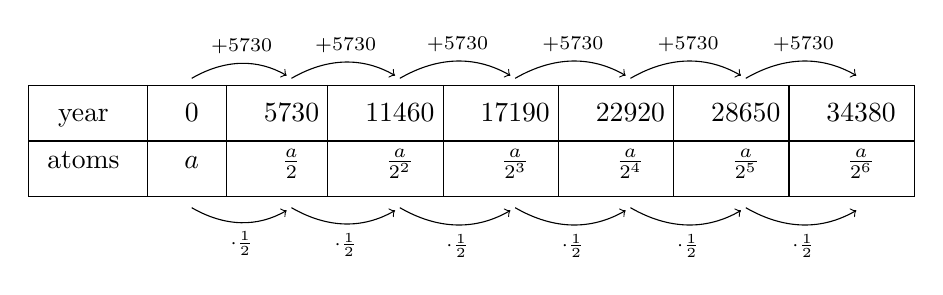
\begin{tikzpicture}
		\matrix[matrix of math nodes,draw, column sep=1em,row sep=.5mm] (mx) {
			\textrm{year} & 0 & 5730 & 11460 & 17190 & 22920 & 28650 & 34380 \\
			\textrm{atoms} & \phantom{\frac{a}{1}}a\phantom{\frac{a}{1}} & \frac{a}{2} & \frac{a}{2^2} & \frac{a}{2^3} & \frac{a}{2^4} & \frac{a}{2^5} & \frac{a}{2^6} \\
		};
		\path[->,shorten >=2pt]
		\foreach \from/\to in {2/3,3/4,4/5,5/6,6/7,7/8} {
			([yshift=2mm]mx-1-\from.north) edge[bend left]
			node[above] {$\scriptstyle+5730$} ([yshift=2mm]mx-1-\to.north)
			([yshift=-2.5mm]mx-2-\from.south) edge[bend right]
			node[below] {$\scriptstyle\cdot\frac{1}{2}$} ([yshift=-2.5mm]mx-2-\to.south)
		};
		\foreach \x in {2,...,8}{
			\draw ([xshift=-1em]mx.north west -| mx-1-\x.west) -- ([xshift=-1em]mx.south west -| mx-1-\x.west);
		};
		\draw (mx.west) -- (mx.east);
	\end{tikzpicture}
\end{figure}
the number of remaining atoms after $x$ is given by the function
\begin{equation*}
	f\left(x\right)=a\cdot 2^{-\frac{x}{5730}}
\end{equation*}
\begin{minipage}{0.48\textwidth}
	\centering
	%\includegraphics[width=\textwidth]{images/decay}
\end{minipage}\hfill
\begin{minipage}{0.48\textwidth}
	\centering
	%\includegraphics[width=\textwidth]{images/kriener_exponential}
\end{minipage}
\begin{tcolorbox}
	An \textbf{exponential function} is a function that can be written as
	\begin{equation*}
		f\left(x\right)=a\cdot b^x
	\end{equation*}
	for some $a\in\mathbb R\setminus\left\{0\right\}$ and some $b>0$.
	We call \ldots
	\begin{itemize}
		\item[] \ldots$a$ the \textbf{initial value} and \ldots
		\item[] \ldots$b$ the \textbf{growth factor} (even if $b<1$).
	\end{itemize}
\end{tcolorbox}
\begin{exercise}
	Show that
	\begin{equation*}
		f\left(x\right)=a\cdot 2^{-\frac{x}{5730}}
	\end{equation*}
	is an exponential function, i.e. find $b$.
	Why do you think $a$ is called initial value?
\end{exercise}
\pagebreak[1]
For a linear function $g\left(x\right)=a\cdot x+b$, we have
\begin{equation*}
	g\left(x+n\right)=a\cdot\left(x+n\right)+b=a\cdot x+b+a\cdot n=g\left(x\right)+a\cdot n.
\end{equation*}
Hence advancing on the $x$ axis by $n$ changes the function value by \textbf{adding} $a\cdot n$.
On the other hand, for an exponential function $f(x)=ab^x$, we have
\begin{equation*}
	f\left(x+n\right)=a\cdot b^{x+n}=a\cdot b^x\cdot b^n=f\left(x\right)\cdot b^n.
\end{equation*}
Advancing on the $x$ axis by $n$ changes the function value by the \textbf{factor} $b^n$.
\begin{exercise}
	These tables contain the values of a function $f\left(x\right)=a\cdot b^x$.
	Complete the tables and determine $a$ and $b$.
	\begin{center}
	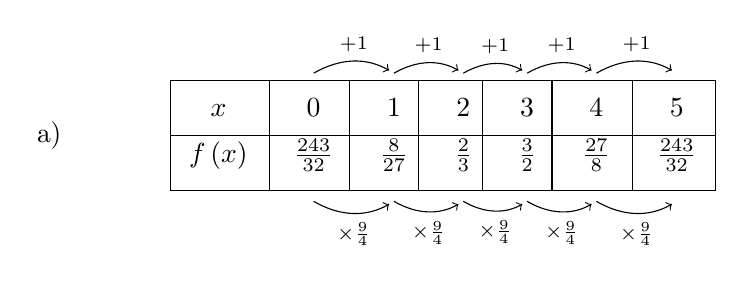
\begin{tikzpicture}
		\node at (-5,0) {a)};
		\matrix[matrix of math nodes,draw, column sep=1em,row sep=.5mm] (mx) {
			x & 0 & 1 & 2 & 3 & 4 & 5 \\
			f\left(x\right) & \frac{243}{32} & \frac{8}{27} & \frac{2}{3} & \frac{3}{2} & \frac{27}{8} & \frac{243}{32} \\
		};
		\path[->,shorten >=2pt]
		\foreach \from/\to in {2/3,3/4,4/5,5/6,6/7} {
			([yshift=2mm]mx-1-\from.north) edge[bend left]
			node[above] {$\scriptstyle+1$} ([yshift=2mm]mx-1-\to.north)
			([yshift=-2.5mm]mx-2-\from.south) edge[bend right]
			node[below] {$\scriptstyle\times\frac{9}{4}$} ([yshift=-2.5mm]mx-2-\to.south)
		};
		\foreach \x in {2,...,7}{
			\draw ([xshift=-1em]mx.north west -| mx-1-\x.west) -- ([xshift=-1em]mx.south west -| mx-1-\x.west);
		};
		\draw (mx.west) -- (mx.east);
	\end{tikzpicture}
	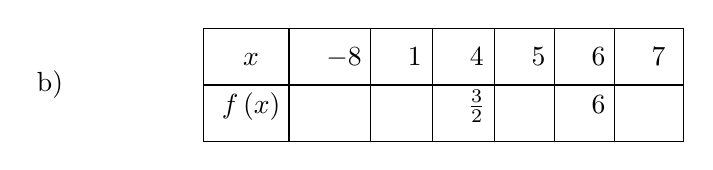
\begin{tikzpicture}
		\node at (-5,0) {b)};
		\matrix[matrix of math nodes,draw, column sep=1em,row sep=.5mm] (mx) {
			x & -8 & 1 & 4 & 5 & 6 & 7 \\
			f\left(x\right) &  &  & \frac{3}{2} & & 6 & \\
		};
%		\path[->,shorten >=2pt]
%		\foreach \from/\to in {2/3,3/4,4/5,5/6,6/7} {
%			([yshift=2mm]mx-1-\from.north) edge[bend left]
%			node[above] {$\scriptstyle+1$} ([yshift=2mm]mx-1-\to.north)
%			([yshift=-2.5mm]mx-2-\from.south) edge[bend right]
%			node[below] {$\scriptstyle\times\frac{9}{4}$} ([yshift=-2.5mm]mx-2-\to.south)
%		};
		\foreach \x in {2,...,7}{
			\draw ([xshift=-1em]mx.north west -| mx-1-\x.west) -- ([xshift=-1em]mx.south west -| mx-1-\x.west);
		};
		\draw (mx.west) -- (mx.east);
	\end{tikzpicture}
	\end{center}
	\renewcommand{\arraystretch}{2.5}
	\setlength{\tabcolsep}{15pt}
	\begin{tabular}{|c|c|c|c|c|c|c|}\hline
		$x$ & 0 & 1 & 2 & 3 & 4 & 5 \\ \hline
		$f\left(x\right)$ & & & $\dfrac{2}{3}$ & $\dfrac{3}{2}$ & & \\ \hline
	\end{tabular}
\end{exercise}
\begin{exercise}
	Consider two points $P=\left(2,12\right)$ and $Q=\left(10,3072\right)$.
	\begin{tasks}
		\task Find the linear function $g\left(x\right)=a\cdot x+b$ that passes through these points.
		\task Find the exponential function $f\left(x\right)=a\cdot b^x$ that passes through these points.
		\task Given two points, is there always a linear function passing through these points?
		\task Given two points, is there always an exponential function passing through these points?
	\end{tasks}
\end{exercise}
%\begin{exercise}
%	Consider again the function
%	\begin{equation*}
%		f\left(x\right)=a\cdot 2^{-\frac{x}{5730}},
%	\end{equation*}
%	where $a$ is now unknown.
%	Suppuse that at time $x=$
%\end{exercise}\newpage
%	\section*{Logarithm}
\textcolor{red}{TODO: relation to exponential equations, change of basis, rules of computation}\newpage
%	\section*{Logarithmic Scale}
Figure~\ref{fig:casesCH} shows the number of infections in Switzerland per day from September to November 2020.
As we are going to see, this is already an example of \textit{exponential growth}.
\begin{figure}[ht]
	\centering
	\includegraphics[width=0.5\textwidth]{images/casesCH}
	\caption{The covid infections in autumn 2020 were growing approximately exponentially.}
	\label{fig:casesCH}
\end{figure}
Looking at the figure, we see that from day 12 to day 36, the number of infections is doubling every 6 days.

\textcolor{red}{TODO: Exponential growth revisited, introduce logarithmically scaled axes}
\end{document}